%% bare_jrnl.tex
%% V1.4
%% 2012/12/27
%% by Michael Shell
%% see http://www.michaelshell.org/
%% for current contact information.
%%
%% This is a skeleton file demonstrating the use of IEEEtran.cls
%% (requires IEEEtran.cls version 1.8 or later) with an IEEE journal paper.
%%
%% Support sites:
%% http://www.michaelshell.org/tex/ieeetran/
%% http://www.ctan.org/tex-archive/macros/latex/contrib/IEEEtran/
%% and
%% http://www.ieee.org/



% *** Authors should verify (and, if needed, correct) their LaTeX system  ***
% *** with the testflow diagnostic prior to trusting their LaTeX platform ***
% *** with production work. IEEE's font choices can trigger bugs that do  ***
% *** not appear when using other class files.                            ***
% The testflow support page is at:
% http://www.michaelshell.org/tex/testflow/


%%*************************************************************************
%% Legal Notice:
%% This code is offered as-is without any warranty either expressed or
%% implied; without even the implied warranty of MERCHANTABILITY or
%% FITNESS FOR A PARTICULAR PURPOSE! 
%% User assumes all risk.
%% In no event shall IEEE or any contributor to this code be liable for
%% any damages or losses, including, but not limited to, incidental,
%% consequential, or any other damages, resulting from the use or misuse
%% of any information contained here.
%%
%% All comments are the opinions of their respective authors and are not
%% necessarily endorsed by the IEEE.
%%
%% This work is distributed under the LaTeX Project Public License (LPPL)
%% ( http://www.latex-project.org/ ) version 1.3, and may be freely used,
%% distributed and modified. A copy of the LPPL, version 1.3, is included
%% in the base LaTeX documentation of all distributions of LaTeX released
%% 2003/12/01 or later.
%% Retain all contribution notices and credits.
%% ** Modified files should be clearly indicated as such, including  **
%% ** renaming them and changing author support contact information. **
%%
%% File list of work: IEEEtran.cls, IEEEtran_HOWTO.pdf, bare_adv.tex,
%%                    bare_conf.tex, bare_jrnl.tex, bare_jrnl_compsoc.tex,
%%                    bare_jrnl_transmag.tex
%%*************************************************************************

% Note that the a4paper option is mainly intended so that authors in
% countries using A4 can easily print to A4 and see how their papers will
% look in print - the typesetting of the document will not typically be
% affected with changes in paper size (but the bottom and side margins will).
% Use the testflow package mentioned above to verify correct handling of
% both paper sizes by the user's LaTeX system.
%
% Also note that the "draftcls" or "draftclsnofoot", not "draft", option
% should be used if it is desired that the figures are to be displayed in
% draft mode.
%
\documentclass[journal]{IEEEtran}
%
% If IEEEtran.cls has not been installed into the LaTeX system files,
% manually specify the path to it like:
% \documentclass[journal]{../sty/IEEEtran}


\usepackage[utf8]{inputenc}


% Some very useful LaTeX packages include:
% (uncomment the ones you want to load)


% *** MISC UTILITY PACKAGES ***
%
%\usepackage{ifpdf}
% Heiko Oberdiek's ifpdf.sty is very useful if you need conditional
% compilation based on whether the output is pdf or dvi.
% usage:
% \ifpdf
%   % pdf code
% \else
%   % dvi code
% \fi
% The latest version of ifpdf.sty can be obtained from:
% http://www.ctan.org/tex-archive/macros/latex/contrib/oberdiek/
% Also, note that IEEEtran.cls V1.7 and later provides a builtin
% \ifCLASSINFOpdf conditional that works the same way.
% When switching from latex to pdflatex and vice-versa, the compiler may
% have to be run twice to clear warning/error messages.






% *** CITATION PACKAGES ***
%
\usepackage{cite}
% cite.sty was written by Donald Arseneau
% V1.6 and later of IEEEtran pre-defines the format of the cite.sty package
% \cite{} output to follow that of IEEE. Loading the cite package will
% result in citation numbers being automatically sorted and properly
% "compressed/ranged". e.g., [1], [9], [2], [7], [5], [6] without using
% cite.sty will become [1], [2], [5]--[7], [9] using cite.sty. cite.sty's
% \cite will automatically add leading space, if needed. Use cite.sty's
% noadjust option (cite.sty V3.8 and later) if you want to turn this off
% such as if a citation ever needs to be enclosed in parenthesis.
% cite.sty is already installed on most LaTeX systems. Be sure and use
% version 4.0 (2003-05-27) and later if using hyperref.sty. cite.sty does
% not currently provide for hyperlinked citations.
% The latest version can be obtained at:
% http://www.ctan.org/tex-archive/macros/latex/contrib/cite/
% The documentation is contained in the cite.sty file itself.






% *** GRAPHICS RELATED PACKAGES ***
%
\ifCLASSINFOpdf
  % \usepackage[pdftex]{graphicx}
  % declare the path(s) where your graphic files are
  % \graphicspath{{../pdf/}{../jpeg/}}
  % and their extensions so you won't have to specify these with
  % every instance of \includegraphics
  % \DeclareGraphicsExtensions{.pdf,.jpeg,.png}
\else
  % or other class option (dvipsone, dvipdf, if not using dvips). graphicx
  % will default to the driver specified in the system graphics.cfg if no
  % driver is specified.
  \usepackage[dvips]{graphicx}
  % declare the path(s) where your graphic files are
  \graphicspath{{figures/}}
  % and their extensions so you won't have to specify these with
  % every instance of \includegraphics
  \DeclareGraphicsExtensions{.eps}
\fi
% graphicx was written by David Carlisle and Sebastian Rahtz. It is
% required if you want graphics, photos, etc. graphicx.sty is already
% installed on most LaTeX systems. The latest version and documentation
% can be obtained at: 
% http://www.ctan.org/tex-archive/macros/latex/required/graphics/
% Another good source of documentation is "Using Imported Graphics in
% LaTeX2e" by Keith Reckdahl which can be found at:
% http://www.ctan.org/tex-archive/info/epslatex/
%
% latex, and pdflatex in dvi mode, support graphics in encapsulated
% postscript (.eps) format. pdflatex in pdf mode supports graphics
% in .pdf, .jpeg, .png and .mps (metapost) formats. Users should ensure
% that all non-photo figures use a vector format (.eps, .pdf, .mps) and
% not a bitmapped formats (.jpeg, .png). IEEE frowns on bitmapped formats
% which can result in "jaggedy"/blurry rendering of lines and letters as
% well as large increases in file sizes.
%
% You can find documentation about the pdfTeX application at:
% http://www.tug.org/applications/pdftex





% *** MATH PACKAGES ***
%
\usepackage[cmex10]{amsmath}
% A popular package from the American Mathematical Society that provides
% many useful and powerful commands for dealing with mathematics. If using
% it, be sure to load this package with the cmex10 option to ensure that
% only type 1 fonts will utilized at all point sizes. Without this option,
% it is possible that some math symbols, particularly those within
% footnotes, will be rendered in bitmap form which will result in a
% document that can not be IEEE Xplore compliant!
%
% Also, note that the amsmath package sets \interdisplaylinepenalty to 10000
% thus preventing page breaks from occurring within multiline equations. Use:
\interdisplaylinepenalty=2500
% after loading amsmath to restore such page breaks as IEEEtran.cls normally
% does. amsmath.sty is already installed on most LaTeX systems. The latest
% version and documentation can be obtained at:
% http://www.ctan.org/tex-archive/macros/latex/required/amslatex/math/

\usepackage{siunitx}
    % Otherwise I can't write the mu symbol for micrometers.
    % It also brings me the \degree symbol, woo!
    % No decibel though, I need to make this one myself.

\usepackage{color}
    % For rendering text is eps_tex files produced by InkScape, even
    % if the text is black.

% *** SPECIALIZED LIST PACKAGES ***
%
%\usepackage{algorithmic}
% algorithmic.sty was written by Peter Williams and Rogerio Brito.
% This package provides an algorithmic environment fo describing algorithms.
% You can use the algorithmic environment in-text or within a figure
% environment to provide for a floating algorithm. Do NOT use the algorithm
% floating environment provided by algorithm.sty (by the same authors) or
% algorithm2e.sty (by Christophe Fiorio) as IEEE does not use dedicated
% algorithm float types and packages that provide these will not provide
% correct IEEE style captions. The latest version and documentation of
% algorithmic.sty can be obtained at:
% http://www.ctan.org/tex-archive/macros/latex/contrib/algorithms/
% There is also a support site at:
% http://algorithms.berlios.de/index.html
% Also of interest may be the (relatively newer and more customizable)
% algorithmicx.sty package by Szasz Janos:
% http://www.ctan.org/tex-archive/macros/latex/contrib/algorithmicx/




% *** ALIGNMENT PACKAGES ***
%
%\usepackage{array}
% Frank Mittelbach's and David Carlisle's array.sty patches and improves
% the standard LaTeX2e array and tabular environments to provide better
% appearance and additional user controls. As the default LaTeX2e table
% generation code is lacking to the point of almost being broken with
% respect to the quality of the end results, all users are strongly
% advised to use an enhanced (at the very least that provided by array.sty)
% set of table tools. array.sty is already installed on most systems. The
% latest version and documentation can be obtained at:
% http://www.ctan.org/tex-archive/macros/latex/required/tools/


% IEEEtran contains the IEEEeqnarray family of commands that can be used to
% generate multiline equations as well as matrices, tables, etc., of high
% quality.




% *** SUBFIGURE PACKAGES ***
%\ifCLASSOPTIONcompsoc
%  \usepackage[caption=false,font=normalsize,labelfont=sf,textfont=sf]{subfig}
%\else
%  \usepackage[caption=false,font=footnotesize]{subfig}
%\fi
% subfig.sty, written by Steven Douglas Cochran, is the modern replacement
% for subfigure.sty, the latter of which is no longer maintained and is
% incompatible with some LaTeX packages including fixltx2e. However,
% subfig.sty requires and automatically loads Axel Sommerfeldt's caption.sty
% which will override IEEEtran.cls' handling of captions and this will result
% in non-IEEE style figure/table captions. To prevent this problem, be sure
% and invoke subfig.sty's "caption=false" package option (available since
% subfig.sty version 1.3, 2005/06/28) as this is will preserve IEEEtran.cls
% handling of captions.
% Note that the Computer Society format requires a larger sans serif font
% than the serif footnote size font used in traditional IEEE formatting
% and thus the need to invoke different subfig.sty package options depending
% on whether compsoc mode has been enabled.
%
% The latest version and documentation of subfig.sty can be obtained at:
% http://www.ctan.org/tex-archive/macros/latex/contrib/subfig/




% *** FLOAT PACKAGES ***
%
%\usepackage{fixltx2e}
% fixltx2e, the successor to the earlier fix2col.sty, was written by
% Frank Mittelbach and David Carlisle. This package corrects a few problems
% in the LaTeX2e kernel, the most notable of which is that in current
% LaTeX2e releases, the ordering of single and double column floats is not
% guaranteed to be preserved. Thus, an unpatched LaTeX2e can allow a
% single column figure to be placed prior to an earlier double column
% figure. The latest version and documentation can be found at:
% http://www.ctan.org/tex-archive/macros/latex/base/


%\usepackage{stfloats}
% stfloats.sty was written by Sigitas Tolusis. This package gives LaTeX2e
% the ability to do double column floats at the bottom of the page as well
% as the top. (e.g., "\begin{figure*}[!b]" is not normally possible in
% LaTeX2e). It also provides a command:
%\fnbelowfloat
% to enable the placement of footnotes below bottom floats (the standard
% LaTeX2e kernel puts them above bottom floats). This is an invasive package
% which rewrites many portions of the LaTeX2e float routines. It may not work
% with other packages that modify the LaTeX2e float routines. The latest
% version and documentation can be obtained at:
% http://www.ctan.org/tex-archive/macros/latex/contrib/sttools/
% Do not use the stfloats baselinefloat ability as IEEE does not allow
% \baselineskip to stretch. Authors submitting work to the IEEE should note
% that IEEE rarely uses double column equations and that authors should try
% to avoid such use. Do not be tempted to use the cuted.sty or midfloat.sty
% packages (also by Sigitas Tolusis) as IEEE does not format its papers in
% such ways.
% Do not attempt to use stfloats with fixltx2e as they are incompatible.
% Instead, use Morten Hogholm'a dblfloatfix which combines the features
% of both fixltx2e and stfloats:
%
% \usepackage{dblfloatfix}
% The latest version can be found at:
% http://www.ctan.org/tex-archive/macros/latex/contrib/dblfloatfix/




%\ifCLASSOPTIONcaptionsoff
%  \usepackage[nomarkers]{endfloat}
% \let\MYoriglatexcaption\caption
% \renewcommand{\caption}[2][\relax]{\MYoriglatexcaption[#2]{#2}}
%\fi
% endfloat.sty was written by James Darrell McCauley, Jeff Goldberg and 
% Axel Sommerfeldt. This package may be useful when used in conjunction with 
% IEEEtran.cls'  captionsoff option. Some IEEE journals/societies require that
% submissions have lists of figures/tables at the end of the paper and that
% figures/tables without any captions are placed on a page by themselves at
% the end of the document. If needed, the draftcls IEEEtran class option or
% \CLASSINPUTbaselinestretch interface can be used to increase the line
% spacing as well. Be sure and use the nomarkers option of endfloat to
% prevent endfloat from "marking" where the figures would have been placed
% in the text. The two hack lines of code above are a slight modification of
% that suggested by in the endfloat docs (section 8.4.1) to ensure that
% the full captions always appear in the list of figures/tables - even if
% the user used the short optional argument of \caption[]{}.
% IEEE papers do not typically make use of \caption[]'s optional argument,
% so this should not be an issue. A similar trick can be used to disable
% captions of packages such as subfig.sty that lack options to turn off
% the subcaptions:
% For subfig.sty:
% \let\MYorigsubfloat\subfloat
% \renewcommand{\subfloat}[2][\relax]{\MYorigsubfloat[]{#2}}
% However, the above trick will not work if both optional arguments of
% the \subfloat command are used. Furthermore, there needs to be a
% description of each subfigure *somewhere* and endfloat does not add
% subfigure captions to its list of figures. Thus, the best approach is to
% avoid the use of subfigure captions (many IEEE journals avoid them anyway)
% and instead reference/explain all the subfigures within the main caption.
% The latest version of endfloat.sty and its documentation can obtained at:
% http://www.ctan.org/tex-archive/macros/latex/contrib/endfloat/
%
% The IEEEtran \ifCLASSOPTIONcaptionsoff conditional can also be used
% later in the document, say, to conditionally put the References on a 
% page by themselves.




% *** PDF, URL AND HYPERLINK PACKAGES ***
%
%\usepackage{url}
% url.sty was written by Donald Arseneau. It provides better support for
% handling and breaking URLs. url.sty is already installed on most LaTeX
% systems. The latest version and documentation can be obtained at:
% http://www.ctan.org/tex-archive/macros/latex/contrib/url/
% Basically, \url{my_url_here}.




% *** Do not adjust lengths that control margins, column widths, etc. ***
% *** Do not use packages that alter fonts (such as pslatex).         ***
% There should be no need to do such things with IEEEtran.cls V1.6 and later.
% (Unless specifically asked to do so by the journal or conference you plan
% to submit to, of course. )


% correct bad hyphenation here
\hyphenation{op-tical net-works semi-conduc-tor}


\begin{document}
%
% paper title
% can use linebreaks \\ within to get better formatting as desired
% Do not put math or special symbols in the title.
\title{Understanding Standing Waves\\by Network Modeling, HIFI Untangled\\and Prospects for Future Instrumentation}
%
%
% author names and IEEE memberships
% note positions of commas and nonbreaking spaces ( ~ ) LaTeX will not break
% a structure at a ~ so this keeps an author's name from being broken across
% two lines.
% use \thanks{} to gain access to the first footnote area
% a separate \thanks must be used for each paragraph as LaTeX2e's \thanks
% was not built to handle multiple paragraphs
%

\author{Bertrand~Delforge,
        John~Pearson,
        Peter~Roelfsema,
        Marc~Verheijen,
        and~Willem~Jellema.% <-this % stops a space
\thanks{B. Delforge, P. Roelfsema and W. Jellema are with SRON Netherlands Institute for Space Research, Groningen, Netherlands e-mail: b.delforge@sron.nl.}% <-this % stops a space
\thanks{B. Delforge, P. Roelfsema and Marc Verheijen are with the Kapteyn Astronomical Institute, Rijksuniversiteit Groningen, Netherlands.}% <-this % stops a space
\thanks{J. Pearson is with the Jet Propulsion Laboratory.}% <-this % stops a space
\thanks{Manuscript received September 9, 2013.}}


% note the % following the last \IEEEmembership and also \thanks - 
% these prevent an unwanted space from occurring between the last author name
% and the end of the author line. i.e., if you had this:
% 
% \author{....lastname \thanks{...} \thanks{...} }
%                     ^------------^------------^----Do not want these spaces!
%
% a space would be appended to the last name and could cause every name on that
% line to be shifted left slightly. This is one of those "LaTeX things". For
% instance, "\textbf{A} \textbf{B}" will typeset as "A B" not "AB". To get
% "AB" then you have to do: "\textbf{A}\textbf{B}"
% \thanks is no different in this regard, so shield the last } of each \thanks
% that ends a line with a % and do not let a space in before the next \thanks.
% Spaces after \IEEEmembership other than the last one are OK (and needed) as
% you are supposed to have spaces between the names. For what it is worth,
% this is a minor point as most people would not even notice if the said evil
% space somehow managed to creep in.



% The paper headers
\markboth{24th International Symposium on Space Terahertz Technology}%
{Delforge \MakeLowercase{\textit{et al.}}: Understanding Standing Waves by Network Modeling}
% The only time the second header will appear is for the odd numbered pages
% after the title page when using the twoside option.
% 
% *** Note that you probably will NOT want to include the author's ***
% *** name in the headers of peer review papers.                   ***
% You can use \ifCLASSOPTIONpeerreview for conditional compilation here if
% you desire.




% If you want to put a publisher's ID mark on the page you can do it like
% this:
%\IEEEpubid{0000--0000/00\$00.00~\copyright~2012 IEEE}
% Remember, if you use this you must call \IEEEpubidadjcol in the second
% column for its text to clear the IEEEpubid mark.



% use for special paper notices
%\IEEEspecialpapernotice{(Invited Paper)}




% make the title area
\maketitle

% As a general rule, do not put math, special symbols or citations
% in the abstract or keywords.
\begin{abstract}
As is the case for many coherent instruments like HIFI, the Heterodyne Instrument for the Far Infrared on the Herschel space observatory, standing waves affect the nominal coupling of the mixer to the local oscillator, calibration black bodies and even the sky.  This results in obvious distortions of the spectral baselines and strongly influences other parameters such as the sideband ratio.  Current uncertainties on HIFI's sideband ratio are about 2--10 percent, depending on the frequency, and are mainly a consequence of an insufficient understanding of the HIFI standing wave phenomenon.

We are developing a systematic and generic methodology for modeling standing waves in coherent optical and quasi-optical systems, using scattering matrices combined with Jones matrices.
This approach allows for a consistent processing of both the phase and polarization information of multi-port networks, and serves as a foundation to combine an arbitrarily large number of networks and predict their interactions.

Our numerical simulations qualitatively reproduce, and therefore explain, many artifacts observed in actual HIFI data.
We are currently improving our technique to produce quantitative predictions.
With HIFI as a hands-on show case for our successful standing wave modeling technique,
we are confident that this generic approach for understanding and predicting standing waves can play a significant role in improving the design of future instruments.
\end{abstract}

% Note that keywords are not normally used for peerreview papers.
\begin{IEEEkeywords}
modeling, standing waves, heterodyne, calibration
\end{IEEEkeywords}






% For peer review papers, you can put extra information on the cover
% page as needed:
% \ifCLASSOPTIONpeerreview
% \begin{center} \bfseries EDICS Category: 3-BBND \end{center}
% \fi
%
% For peerreview papers, this IEEEtran command inserts a page break and
% creates the second title. It will be ignored for other modes.
\IEEEpeerreviewmaketitle



\section{Introduction}
% The very first letter is a 2 line initial drop letter followed
% by the rest of the first word in caps.
% 
% form to use if the first word consists of a single letter:
% \IEEEPARstart{A}{demo} file is ....
% 
% form to use if you need the single drop letter followed by
% normal text (unknown if ever used by IEEE):
% \IEEEPARstart{A}{}demo file is ....
% 
% Some journals put the first two words in caps:
% \IEEEPARstart{T}{his demo} file is ....
% 
% Here we have the typical use of a "T" for an initial drop letter
% and "HIS" in caps to complete the first word.
% You must have at least 2 lines in the paragraph with the drop letter
% (should never be an issue)
\IEEEPARstart{T}{he} HIFI instrument on the Herschel Space Observatory~\cite{AA_518_L1} is a heterodyne receiver that operates at frequencies between \SI{480}{\giga\hertz} and \SI{1910}{\giga\hertz},
producing spectra with a resolution ranging from \SI{1}{\mega\hertz} to \SI{125}{\kilo\hertz}~\cite{AA_518_L6}.
This high frequency resolution enables the astronomers to study the chemistry of a wide range of phenomena, from planetary atmospheres to star forming regions.

At such a high resolution, the thermal noise of the astronomical source, the calibration black bodies and the local oscillator (LO) qualify as ``narrow band Gaussian noise signals''~\cite{siegman1986lasers}.
They have a coherence time~$\tau$ equal to the inverse of their bandwidth~$\tau=1/\Delta f$.
A bandwidth of~\SI{1}{\mega\hertz} results in a coherence time of~\SI{1}{\micro\second} equivalent to a coherence length of~\SI{300}{\meter}.
This is a hundred times the longest distance inside HIFI.
Therefore, in HIFI, the signals from the LO, the calibration sources and the sky are coherent.

In a coherent system, interferences can appear.
Interference inside electromagnetic cavities give rise to standing waves which trap energy inside these cavities.
Destructive interferences in the plane of the mixer prevent the mixer from detecting some of the signal.
In other words, the mixer coupling of the incoming signals is modulated by these standing waves.

Figure~\ref{fig:scatter_real_data} illustrates this phenomenon for a very subtle case
(the calibration paper by Roelfsema et al.\ \cite{AA_537_A17} illustrates more obvious ones).
HIFI observed a single emission feature from a galactic source for 25 local oscillator frequencies.
If there were no standing waves, or if the standing waves were perfectly calibrated out, then all these line profiles would overlap within the noise.
Instead, their peak intensity is scattered by more than the expected noise.
This scatter is due to standing waves that are ignored by the calibration: each LO frequency requires a specific tuning of the diplexer, which changes the optical paths, which changes the periods of the standing waves, which changes the mixer coupling to the sky, LO and calibration loads.
This case is a subtle one: each of these 25 spectra looks individually clean from standing wave modulations (no apparent periodic distortion of the spectrum), only their comparison reveals the effect of standing waves.
Standing waves introduce a systematic uncertainty that cannot be reduced by integrating longer.
When an observation is taken at one LO frequency only, the astronomer has little to no way of knowing how much standing waves distort the line.

Our goal is to model the instrument to a level which allows to accurately predict the effect of the standing waves, and include a correction of their effect in the calibration scheme of HIFI.

%=============================================================================

\section{Modeling standing waves}

\subsection{Principle}
Our method is inspired from laser and circuit theory: we deal with discrete inputs and outputs rather than, for example, a spatial description of the fields.
A system like the Focal Plane Unit of HIFI comprises a few dozens of optical elements~\cite{jackson2002hifi}, referred in the literature as ``networks''~\cite{siegman1986lasers}: wire grid polarizers, roof-top mirrors, horns, attenuators, free space, all having one or more input and output.
All these networks interact together two by two since there exists at least one optical path between each pair or networks.
The number of interactions in the system increases faster than the square of the number of networks.
One way to solve a system's reaction to a set of input would be to propagate the inputs from network to network, back and forth, until the fields appear to converge to a steady state.
Instead, we propose a method to reduce the number of networks without losing any information, in a way that can be compared to calculating the equivalent impedance of an electric circuit.
Our model computes the scattering matrix of the network equivalent to the whole system.
Then, knowing how the system reacts to an input is merely a matter of multiplying its scattering matrix with a vector of inputs to get a vector of outputs.
Note that if two inputs are not phase-locked to each other (for example, the LO and the sky), they must be multiplied by the scattering matrix separately, and the two results must be squared (converted into power) before being added.

\begin{figure}
    \centering
    % CO 9-8 line of NCG7538-IRS1 observed on 21-02-2010.
    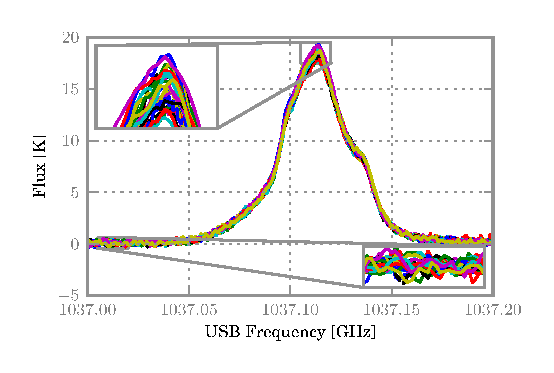
\includegraphics{obsid_5000352C}
    \caption{
    The plot shows the same extragalactic emission feature observed by HIFI at 25 different LO frequencies in its band 4a.
    The standard deviation of the scatter on the line peak is three times greater than the expected noise (inset plots at $\times 4$ magnification).
    }%
    \label{fig:scatter_real_data}
\end{figure}

Scattering matrices \cite{siegman1986lasers} model the transfer of power or field from one side (port) of a network to another (figure~\ref{fig:ports}).

\begin{figure}
    \centering
    \input{figures/scattering_matrix_notations.eps_tex}
    \caption{A 4-ports network showing 4 inputs $a_i$ and four outputs $b_i$.  For example, this network could be a wire grid polarizer or a semi-transparent mirror, both acting as beam splitters.}%
    \label{fig:ports}
\end{figure}

Equation~\ref{eq:scattering_matrix} presents the scattering matrix $S$ that models the relation between a vector of inputs $a$ and a vector of outputs $b$ for a $n$-ports network.
The diagonal contains the reflections terms and the rest contains the transmissions.
\begin{align}
    b &= S a
    &
    \begin{pmatrix}
        b_1\\
        b_2\\
        \vdots\\
        b_n
    \end{pmatrix}
    &=
    \begin{pmatrix}
        S_{1, 1} & S_{1, 2} & \cdots & S_{1, n} \\
        S_{2, 1} & S_{2, 2} & \cdots & S_{2, n} \\
        \vdots   & \vdots   & \ddots & \vdots   \\
        S_{n, 1} & S_{n, 2} & \cdots & S_{n, n}
    \end{pmatrix}
    \begin{pmatrix}
        a_1\\
        a_2\\
        \vdots\\
        a_n
    \end{pmatrix}
    \label{eq:scattering_matrix}
\end{align}
The standard way to include the polarization into a scattering matrix is to double (local reference frame: horizontal and vertical directions) or triple (global reference frame: $x$, $y$ and $z$ directions) its number of ports.
For our model, we chose a different approach that allows us consider a polarized field as a single entity instead of two or three, and keep the number of ports to a minimum.
For this, we adapt the traditional scattering matrix formalism to our need:
the elements~$S_{i, j}$ of the scattering matrix~$S$ are not scalars, but Jones matrices.

Jones matrices model the transfer of amplitude and phase from one polarization to another \cite{hecht2002optics}.
In~\eqref{eq:jones_matrix_short}, the polarized input field $e_i$ is related to the polarized output field~$e_o$ by the Jones matrix $J$.
$e_i$ and $e_o$ are called ``Jones vectors''.
\begin{equation}
    % Small form.
    e_o = J e_i
    \label{eq:jones_matrix_short}
\end{equation}
The components of the Jones vectors are phasors: complex numbers that encode the amplitude and phase of the field along different axes.
The components of the Jones matrices are also complex numbers, these encode changes in amplitude and phase.

Equation~\eqref{eq:jones_matrix_2d} presents the traditional form of Jones vectors and matrices.
\begin{equation}
    % Jones matrix in 2D.
    \begin{pmatrix}
        e_{o, h}\\
        e_{o, v}
    \end{pmatrix}
    =
    \begin{pmatrix}
        J_{h, h}   &   J_{h, v} \\
        J_{v, h}   &   J_{v, v}
    \end{pmatrix}
    \begin{pmatrix}
        e_{i, h}\\
        e_{i, v}
    \end{pmatrix}
    \label{eq:jones_matrix_2d}
\end{equation}
The field is seen as the superposition of a horizontal and a vertical component, both linearly polarized.
The phase difference between these components determines the handedness and the ellipticity of the polarization of the field.
Although very useful for many applications, these Jones matrices and vectors have limitations.

\begin{figure*} % The star version creates a float that spans two columns.
    \centering
    \input{figures/cascading_example.eps_tex}
    \caption{
    A system comprising several networks connected by one port can be reduced to a single equivalent network.
    This is done by recursively combining networks two by two until there is only one network left.
    This example presents a HIFI diplexer unit; its Martin-Puplett interferometer contains two rooftop mirrors (pentagons) and a wire grid polarizer (dotted line) separated by free space (rectangles); its purpose is to align the polarization of the LO and the sky signals in order to couple both to the mixer (crossed circle) which produces the intermediate frequency (IF).
    }%
    \label{fig:cascading_example}
\end{figure*}

First, the field is always expressed in a local reference frame: the horizontal and vertical directions are valid for one beam only and may change after any reflection or refraction.
Therefore, to completely describe a field, the Jones vector is not enough since one needs to keep track of the orientation of its reference frame with three angles, a quaternion or a rotation matrix.

Second, the horizontal and vertical directions are normal to each other and to the direction of propagation.
This limits us to modeling either TE or TM waves\footnote{transverse electric, transverse magnetic} depending on whether the Jones vector represents the electric or the magnetic field.
However, this cannot model hybrid waves, in which both the electric and the magnetic field can have a component along the direction of propagation.
Therefore, this cannot model propagation in a birefringent material.
One way to accommodate this is to relax the constraint of orthogonality of the reference frame, allowing for the horizontal and vertical directions to have a component along the direction of propagation.
If we do this, then the full description of the field gets even more complicated as we need to carry along, not just the orientation of its reference frame, but the full description of that non-Cartesian reference frame.

Instead, we can express all the fields in a common global Cartesian reference frame, essentially extending Jones calculus from two to three dimensions, as illustrated in~\eqref{eq:jones_matrix_3d}.
\begin{equation}
    % Jones matrix in 3D.
    \begin{pmatrix}
        e_{o, x}\\
        e_{o, y}\\
        e_{o, z}
    \end{pmatrix}
    =
    \begin{pmatrix}
        J_{x, x}   &   J_{x, y}   &   J_{x, z} \\
        J_{y, x}   &   J_{y, y}   &   J_{y, z} \\
        J_{z, x}   &   J_{z, y}   &   J_{z, z}
    \end{pmatrix}
    \begin{pmatrix}
        e_{i, x}\\
        e_{i, y}\\
        e_{i, z}
    \end{pmatrix}
    \label{eq:jones_matrix_3d}
\end{equation}


\begin{figure}
    \centering
    \input{figures/cascading.eps_tex}
    \caption{\label{fig:cascading}Two networks P~and~Q connected by one port are equivalent to a network S.}
\end{figure}

As shown on figure~\ref{fig:cascading}, two networks~P and~Q connected by one port can be seen as a single equivalent network~S.
Our model can compute the scattering matrix of~S from the scattering matrices of~P and~Q for any P~and~Q connected by any port.
The scattering matrix of S takes into account the infinite reflections on the ports by which P~and~Q are connected.

Once we have this method to compute~S from~P and~Q, we apply it recursively to get the scattering matrix of the whole system.
This is illustrated by figure~\ref{fig:cascading_example}, where we use a HIFI diplexer unit as an example and reduce it to a single network.



Our method is recursive but not iterative: it passes over each network only once.
Once the scattering matrix of the whole system is calculated, we have direct access to the steady state of that system.

The detail of the mathematics and algorithms used in this model falls out of the scope of this paper and shall be presented in a later publication~\cite{delforge_2014_phdthesis}.

% needed in second column of first page if using \IEEEpubid
%\IEEEpubidadjcol

%-----------------------------------------------------------------------------

\subsection{Simplifications}

HIFI operates in the submillimeter regime where the wavelength is of the same order as the dimensions of the networks.
We could use quasi optics to properly account for the diffraction of the beams \cite{goldsmith1998quasioptical}.
However, our model assumes plane, and therefore single-mode, waves.
The plane-wave hypothesis is acceptable at a first order because the networks are placed at the waist of the beams where the wave front is plane.
Furthermore, the discrepancies due to these simplifications can be abstracted, withing reason, by physical parameters in our model.
For example, if a higher mode does not couple to a mixer, then its power is --for all practical purpose-- lost, and therefore a term of loss can model it.

If needed, our model can be extended to higher order modes.
This can be done by adding components to the Jones vectors/matrices, or by adding an additional layer of matrices between the scattering matrix and the Jones matrix, which would take care of the transfer of power between modes.

\subsection{Typical networks.}
Most typical networks can be easily modeled at the first order;
we generate their scattering matrices with parameters such as refractive index, thickness, orientation in space, attenuation, etc.
Our model can compute the scattering matrices of dielectric thin films, reflective surfaces and interfaces, rooftop mirrors, horns, free space (or space of any refractive index), attenuators and black bodies (which are not totally black).

Wire grid polarizers are much more difficult to model; we adapted the work of Martin Houde et al.\ \cite{houde_2001} to our matrix format.

%=============================================================================

\section{Qualitative achievement}



A typical HIFI observation consists in four integrations: one on the astronomical source, one on a reference position in the sky, and two internal black bodies (``Hot'' and ``Cold'') used for intensity calibration.
The details of the intensity calibration of HIFI are described in the ALMA Memo 442.1 by Volker Ossenkopf \cite{ossenkopf2002intensity}.
A traditional calibration scheme using these four integrations would follow~\eqref{eq:std_calibration}.
\begin{equation}
    \text{flux}_\text{source} = 
    \text{constant}
    \times
    \frac{\text{source} - \text{reference}}{\text{hot} - \text{cold}}
    \label{eq:std_calibration}
\end{equation}
In~\eqref{eq:std_calibration}, the subtractions correct for constant terms such as the local oscillator noise, the division corrects for the bandpass of the system and the constant converts the CCD counts into physical units such as Jansky.
This is not sufficient for HIFI.
HIFI is special in that it is double-sideband: to every channel of the spectrometer correspond two frequencies, one from the lower sideband~``LSB'' and one from the upper sideband~``USB''.
The output of the mixer at the intermediate frequency~``IF'' is a weighted sum of the signals at the LSB and USB frequencies~\eqref{eq:weighted_sum}.
\begin{equation}
    J_\text{IF} = G_\text{LSB} J_\text{LSB} + G_\text{USB} J_\text{USB}
    \label{eq:weighted_sum}
\end{equation}
In~\eqref{eq:weighted_sum}, $J$ refers to a power and $G$ to a gain.
Standing waves, being frequency-dependent, affect the lower and upper sidebands differently.
This results in an imbalanced coupling of the two sidebands to the mixer: $G_\text{LSB} \neq G_\text{USB}$.
The problem is the following: the spectral lines are narrow features that appear in one sideband only while the continuum is present in both sidebands.
If one does not know~$G_\text{LSB}$ and~$G_\text{USB}$, one cannot properly retrieve the amplitude of the line from $J_\text{IF}$.

\begin{figure}
    \centering
    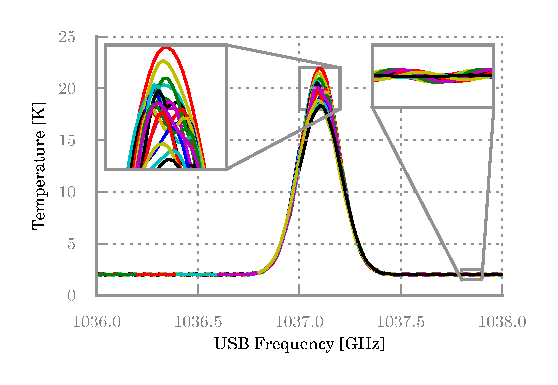
\includegraphics[width=\columnwidth]{bb-on_corrected-2}
    \caption{Simulated line with standard HIFI calibration for 25 LO frequencies.
    Standing waves introduce a weak periodic modulation of the baseline and a strong scatter of the peak intensity of the line.}%
    \label{fig:calibrated_std}
\end{figure}

\begin{figure}
    \centering
    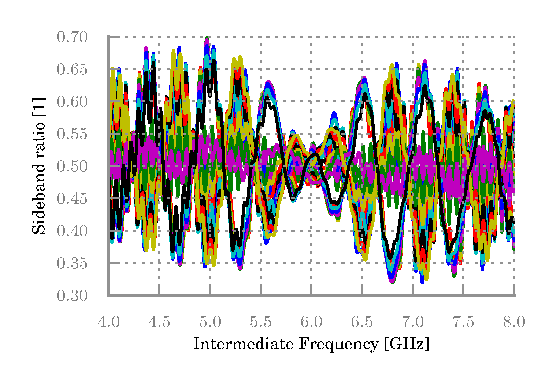
\includegraphics[width=\columnwidth]{sbr}
    \caption{Simulated sideband ratio for a diplexer band of HIFI at 25 different LO~frequencies.
    The sideband ratio varies quickly over the intermediate frequency, as several standing wave patterns beat and modulate each other.
    For some LO frequencies, the sideband ratio varies considerably ($\pm 0.15$), while for some others, it remains closer to the ideal value ($\pm 0.05$).}%
    \label{fig:sbr}
\end{figure}

\begin{figure}
    \centering
    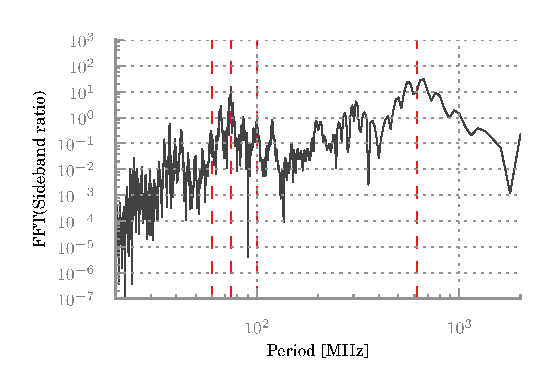
\includegraphics[width=\columnwidth]{sbr_fft}
    \caption{Fourier transform of a simulated sideband ratio for a diplexer band of HIFI.
    The vertical lines mark expected peaks: mixer--cold-black-body at \SI{60}{\mega\hertz}, mixer--hot-black-body at \SI{75}{\mega\hertz}, mixer--LO at \SI{100}{\mega\hertz}, mixer--rooftop-mirror at \SI{620}{\mega\hertz}.
    The two peaks around \SI{620}{\mega\hertz} are real, they are caused by the~\SI{12}{\centi\meter} difference in pathlength between the two rooftop mirrors of the diplexer units.  All the other peaks are doubled for this reason, although this is hardly visible at that scale.}
    \label{fig:sbr_fft}
\end{figure}

\begin{figure}
    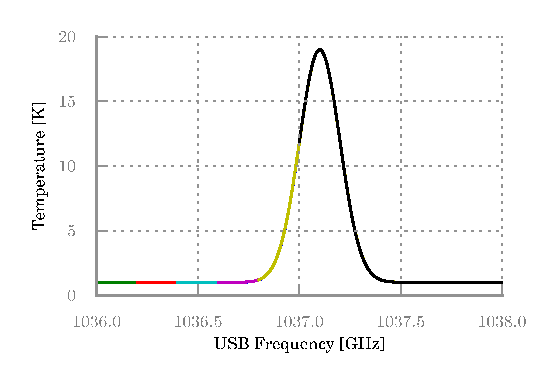
\includegraphics[width=\columnwidth]{bb-on_corrected-3}
    \caption{Simulated line for 25 LO frequencies, with a calibration scheme that uses the sideband ratio provided by the model.  The 25 plots overlap within numerical noise.}
    \label{fig:calibrated_sbr}
%    \caption{\label{fig:calibrated}Simulated spectra.
%    Each LO tuning brings its own set of standing waves that modulate the couplings to the different sources.
%    Without knowledge of these couplings, the calibration is not perfect.
%    The model gives us some information that allows us to properly calibrate out all the standing waves.}
\end{figure}

Disentangling the sidebands requires some a-priori knowledge of the instrument.
In absence of that knowledge, we have to make assumptions.
In Ossenkopf's Memo \cite{ossenkopf2002intensity}, it is assumed that the standing waves are the same, or are very similar, on the Hot and Cold integrations even though the optical paths are different.
We know that this assumption does not always hold because some HIFI spectra show ripples that have periods corresponding to standing waves between the mixer and the black bodies; the calibration did not cancel them out.
By calculating the effect of standing waves on the coupling of the mixers to the source, our model can give us $G_\text{LSB}$ and~$G_\text{USB}$ and relieve us from the need of making assumptions.

Using the method presented in this article, we model the optical part of HIFI, that is the networks between the sky and the mixers.
In order to reproduce the behavior illustrated in figure~\ref{fig:scatter_real_data}, we present four sources to that model: a perfect Gaussian line of~\SI{18}{\kelvin} on top of a~\SI{1}{\kelvin} continuum, a reference source with no signal (no continuum no line), and two calibration black bodies at \SI{10}{\kelvin} and \SI{100}{\kelvin}.
Each of these integrations also receives power from the local oscillator, approximated with a~\SI{120}{\kelvin} black body.

With the standard calibration~\eqref{eq:std_calibration}, which ignores standing waves, the result is given in figure~\ref{fig:calibrated_std}

Figure~\ref{fig:calibrated_std} shows that our model properly reproduces the scatter seen on real data (figure~\ref{fig:scatter_real_data}).
It also reveals the effect of standing waves on the baseline.
The ripples on the baseline are not visible on figure~\ref{fig:scatter_real_data} because the noise level is high (a strong line does not need a long integration time); spectra of weak lines have a lower noise level and show ripples on the baseline.

Our model gives us the information we need to calibrate our data: $G_\text{LSB}$ and $G_\text{USB}$.
We define the sideband ratio with equation~\eqref{eq:sbr}, it is a measure of the coupling imbalance between the two sidebands.
Its ideal value is 0.5; above 0.5, the channel is USB-dominated, and under 0.5 it is LSB-dominated.
\begin{equation}
    \text{sideband ratio}
    =
    \frac{G_\text{USB}}{G_\text{LSB} + G_\text{USB}}
    \label{eq:sbr}
\end{equation}
The sideband ratios corresponding to our simulation of the integration on the hot black body, for 25 local oscillator frequencies, are plotted on figure~\ref{fig:sbr}.

The \SI{620}{\mega\hertz}-wide periodic modulation of the sideband ratio (figure~\ref{fig:sbr}) comes from the standing wave between the mixers and the closest roof-top mirrors of the diplexer assemblies (described in Jackson et al.\ \cite{jackson2002hifi}, using the principles of Martin-Puplett inteferometers~\cite{martin1982polarizing}).
The wide envelop results from the fact that the diplexer tuning is optimal at the center of the bandwidth and degrades on the edges.
A Fourier transform of these plots (figure~\ref{fig:sbr_fft}) reveals many short period patterns.
The short-period features correspond to standing waves in the cavities formed by the mixers and
the local oscillator ($\approx$~\SI{100}{\mega\hertz}),
cold black body ($\approx$~\SI{60}{\mega\hertz}) or
hot black body ($\approx$~\SI{75}{\mega\hertz}).
The cold and hot standing waves in this simulation do not correspond to that of the real instrument (which are~\SI{98}{\mega\hertz} for cold and~\SI{92}{\mega\hertz} for hot): this is deliberate, our model can reproduce the exact cold and hot standing waves, but in this case their periods are so close that it is difficult to tell them apart and track their contribution by visual inspection.

To complicate the situation, each short-period pattern appears twice, at two slightly different periods, because the two rooftop mirrors of the diplexer assemblies produce two slightly different optical path lengths.

Finally, there is some ``cross-talk'' between the two polarizations: the vertical mixer sees the horizontal one and vice-versa.
This is due to imperfections of the wire grid polarizers.



Our model computes all these effects at once.
Using this information, we can properly calibrate our simulated spectrum, as illustrated in figure~\ref{fig:calibrated_sbr}.
It must be noted that solving the calibration equation requires to know the spectrum of the local oscillator in the lower and upper side band.
Indeed, the contribution of the local oscillator is not canceled by the $\text{hot}-\text{cold}$ subtraction since it is affected by different standing waves for hot and for cold.

The framework presented in this article is able to qualitatively predict the behavior of coherent systems as complex as HIFI.
It can be applied to any coherent instrument.

Reaching a quantitative level of prediction is possible.
It requires a precise modeling of each network of the system.
The algorithm that combines the networks together and predicts their interactions is, as we have demonstrated, already in place.




%=============================================================================

\section{Conclusion}
We have designed and implemented a framework to model the interferences, and therefore the standing waves, in any coherent instrument.

This model qualitatively reproduces and explains a wide range of phenomena observed in HIFI data.
This makes it a powerful tool to assist the design of future instruments.
Its applications are not limited to astronomy; for example, this method can be applied to optimize cavity ring-down spectrometers.
It is not restricted to the submillimetric domain either, as any coherent system (optical lasers for instance) can be studied with this framework.

By modeling more accurately the individual networks of HIFI, we are expecting to reproduce its behavior at a quantitative level.
If successful, this processing would find its place in the calibration pipeline of HIFI, improving significantly the accuracy of the data taken during its mission.


%=============================================================================
% An example of a floating figure using the graphicx package.
% Note that \label must occur AFTER (or within) \caption.
% For figures, \caption should occur after the \includegraphics.
% Note that IEEEtran v1.7 and later has special internal code that
% is designed to preserve the operation of \label within \caption
% even when the captionsoff option is in effect. However, because
% of issues like this, it may be the safest practice to put all your
% \label just after \caption rather than within \caption{}.
%
% Reminder: the "draftcls" or "draftclsnofoot", not "draft", class
% option should be used if it is desired that the figures are to be
% displayed while in draft mode.
%
%\begin{figure}[!t]
%\centering
%\includegraphics[width=2.5in]{myfigure}
% where an .eps filename suffix will be assumed under latex, 
% and a .pdf suffix will be assumed for pdflatex; or what has been declared
% via \DeclareGraphicsExtensions.
%\caption{Simulation Results.}
%\label{fig_sim}
%\end{figure}

% Note that IEEE typically puts floats only at the top, even when this
% results in a large percentage of a column being occupied by floats.


% An example of a double column floating figure using two subfigures.
% (The subfig.sty package must be loaded for this to work.)
% The subfigure \label commands are set within each subfloat command,
% and the \label for the overall figure must come after \caption.
% \hfil is used as a separator to get equal spacing.
% Watch out that the combined width of all the subfigures on a 
% line do not exceed the text width or a line break will occur.
%
%\begin{figure*}[!t]
%\centering
%\subfloat[Case I]{\includegraphics[width=2.5in]{box}%
%\label{fig_first_case}}
%\hfil
%\subfloat[Case II]{\includegraphics[width=2.5in]{box}%
%\label{fig_second_case}}
%\caption{Simulation results.}
%\label{fig_sim}
%\end{figure*}
%
% Note that often IEEE papers with subfigures do not employ subfigure
% captions (using the optional argument to \subfloat[]), but instead will
% reference/describe all of them (a), (b), etc., within the main caption.


% An example of a floating table. Note that, for IEEE style tables, the 
% \caption command should come BEFORE the table. Table text will default to
% \footnotesize as IEEE normally uses this smaller font for tables.
% The \label must come after \caption as always.
%
%\begin{table}[!t]
%% increase table row spacing, adjust to taste
%\renewcommand{\arraystretch}{1.3}
% if using array.sty, it might be a good idea to tweak the value of
% \extrarowheight as needed to properly center the text within the cells
%\caption{An Example of a Table}
%\label{table_example}
%\centering
%% Some packages, such as MDW tools, offer better commands for making tables
%% than the plain LaTeX2e tabular which is used here.
%\begin{tabular}{|c||c|}
%\hline
%One & Two\\
%\hline
%Three & Four\\
%\hline
%\end{tabular}
%\end{table}


% Note that IEEE does not put floats in the very first column - or typically
% anywhere on the first page for that matter. Also, in-text middle ("here")
% positioning is not used. Most IEEE journals use top floats exclusively.
% Note that, LaTeX2e, unlike IEEE journals, places footnotes above bottom
% floats. This can be corrected via the \fnbelowfloat command of the
% stfloats package.







% if have a single appendix:
%\appendix[Proof of the Zonklar Equations]
% or
%\appendix  % for no appendix heading
% do not use \section anymore after \appendix, only \section*
% is possibly needed

% use appendices with more than one appendix
% then use \section to start each appendix
% you must declare a \section before using any
% \subsection or using \label (\appendices by itself
% starts a section numbered zero.)
%


\appendices

\section*{Acknowledgment}


The authors would like to thank...


% Can use something like this to put references on a page
% by themselves when using endfloat and the captionsoff option.
\ifCLASSOPTIONcaptionsoff
  \newpage
\fi



% trigger a \newpage just before the given reference
% number - used to balance the columns on the last page
% adjust value as needed - may need to be readjusted if
% the document is modified later
\IEEEtriggeratref{5}
% The "triggered" command can be changed if desired:
%\IEEEtriggercmd{\enlargethispage{-5in}}

% references section

% can use a bibliography generated by BibTeX as a .bbl file
% BibTeX documentation can be easily obtained at:
% http://www.ctan.org/tex-archive/biblio/bibtex/contrib/doc/
% The IEEEtran BibTeX style support page is at:
% http://www.michaelshell.org/tex/ieeetran/bibtex/
\bibliographystyle{IEEEtran}
% argument is your BibTeX string definitions and bibliography database(s)
\bibliography{IEEEabrv,bibliography}
%
% <OR> manually copy in the resultant .bbl file
% set second argument of \begin to the number of references
% (used to reserve space for the reference number labels box)
%\begin{thebibliography}{1}
%
%\bibitem{IEEEhowto:kopka}
%H.~Kopka and P.~W. Daly, \emph{A Guide to \LaTeX}, 3rd~ed.\hskip 1em plus
%  0.5em minus 0.4em\relax Harlow, England: Addison-Wesley, 1999.
%
%\end{thebibliography}

% You can push biographies down or up by placing
% a \vfill before or after them. The appropriate
% use of \vfill depends on what kind of text is
% on the last page and whether or not the columns
% are being equalized.

%\vfill

% Can be used to pull up biographies so that the bottom of the last one
% is flush with the other column.
%\enlargethispage{-5in}



% that's all folks
\end{document}
